\documentclass{fict}

\usepackage{tikz}
\usetikzlibrary{arrows.meta,positioning,shapes.geometric}
\usepackage{tabularx}

\addbibresource{references.bib}
\ExecuteBibliographyOptions{maxbibnames=99}

% Glossary of mathematical symbols used in the dissertation.
% Reference entries with \gls{key}. Add as you introduce new symbols.

\newglossaryentry{H}
{
    name=\(H\),
    description={Homography matrix that maps image-plane pixel coordinates to real-world pitch coordinates},
    sort=H
}

% Acronyms used throughout the dissertation.
% Reference them with \gls{key} (first use expands; later uses abbreviate).
% Add new entries as you introduce them in the text.

\newacronym[description={Final Year Project}]{fyp}{FYP}{Final Year Project}
\newacronym[description={You Only Look Once --- a real-time object detection model family}]{yolo}{YOLO}{You Only Look Once}
\newacronym[description={Convolutional Neural Network}]{cnn}{CNN}{Convolutional Neural Network}
\newacronym[description={Random Sample Consensus --- a robust model-fitting algorithm}]{ransac}{RANSAC}{Random Sample Consensus}
\newacronym[description={Singular Value Decomposition}]{svd}{SVD}{Singular Value Decomposition}
\newacronym[description={Video Assistant Referee}]{var}{VAR}{Video Assistant Referee}
\newacronym[description={Direct Linear Transform --- algorithm for solving the homography estimation system}]{dlt}{DLT}{Direct Linear Transform}
\newacronym[description={Hue, Saturation, Value --- a cylindrical colour model}]{hsv}{HSV}{Hue, Saturation, Value}
\newacronym[description={Red, Green, Blue --- the standard additive colour model for digital images}]{rgb}{RGB}{Red, Green, Blue}
\newacronym[description={International Football Association Board --- the body that maintains the Laws of the Game}]{ifab}{IFAB}{International Football Association Board}
\newacronym[description={harmonic mean of precision and recall}]{fone}{F1}{F-measure}
\newacronym[description={Median Absolute Deviation --- a robust spread estimator resistant to outliers}]{mad}{MAD}{Median Absolute Deviation}
\newacronym[description={Kanade--Lucas--Tomasi --- an optical flow feature tracker}]{klt}{KLT}{Kanade--Lucas--Tomasi}


\title{A Computer Vision-Based Approach for Event Detection in Football Videos}
\author{Aidan Cristina}
\supervisor{Prof.\ Ing.\ Carl James Debono}
\degreename{B.Sc.\ (Hons.) Computing Science}
\titledate{June 2026}

\begin{document}

\frontmatter{}
\pagestyle{pageNumbersOnly}

\input{content/title.tex}
\chapter*{Abstract}
\addcontentsline{toc}{chapter}{Abstract}

Automation in football decisions attempts to reduce subjective error to protect the integrity of the game's most crucial moments. However, the infrastructure required to support offside decisions remains unavailable outside the elite tier of the sport. This final year project investigates the feasibility of automated offside detection from broadcast video alone, through the design and evaluation of a modular computer vision pipeline.

The pipeline operates on broadcast clips drawn from the publicly available SoccerNet dataset, covering thousands of games across the top five European Leagues and even the UEFA Champions League up until the 2016/2017 season. For each offside clip in each downloaded game, the keyframe corresponding to the moment of the pass is manually selected via a browser-based annotation interface. Players are then detected using a YOLO-based object detector, and team identification is done through clustering kit colours in Lab colour space using K-Means. A homography between the broadcast image plane and a real-world pitch coordinate system is estimated using RANSAC over manually picked relevant pitch landmarks, allowing every player's position to be projected onto a metric pitch. The offside condition is then evaluated geometrically by comparing the attacking player against the deepest outfield defender along the direction of attack.

One hundred and fifty offside events were processed and compared against the annotations provided by SoccerNet. Of these, 128 verdicts (85.3\%) agreed with the dataset annotations. Since the annotations reflect the match official's judgement rather than a geometric ground truth, disagreements may originate from system error or from official error; the two cannot be distinguished without independent measurement. Agreement rose to 91.3\% for the 92 events where the measured margin was above 0.5\,m, the threshold below which both human judgement and the system's geometric precision become questionable, demonstrating that broadcast-only offside detection is feasible on representative footage. The principal sources of system error include occasional team misidentification and imprecision in the estimated homography.

The major computational expense of the automation is the two YOLO11x-seg inference passes per event, which take around 90\,ms on commodity GPU hardware. The main remaining obstacles to fully automated deployment are the manual keyframe selection and landmark picking stages, which are identified as the primary directions for future work.
\chapter*{Acknowledgements}
\addcontentsline{toc}{chapter}{Acknowledgements}

I would like to express my sincere gratitude to my supervisor, Prof.\ Ing.\ Carl James Debono, for his guidance, support, and constructive feedback throughout the duration of this Final Year Project.

Acknowledgement is also due to the SoccerNet project for making broadcast match footage freely available for academic research; the present work would not have been possible without this dataset.

Finally, I wish to thank my family and friends for their unwavering encouragement and support throughout the course of my studies.

\clearpage{}

\phantomsection
\addcontentsline{toc}{chapter}{Contents}
\tableofcontents{}
\clearpage{}

\listoffigures{}
\addcontentsline{toc}{chapter}{List of Figures}
\clearpage{}

\listoftables{}
\addcontentsline{toc}{chapter}{List of Tables}
\clearpage{}

\printglossary[type=\acronymtype,nonumberlist,title=List of Abbreviations]
\addcontentsline{toc}{chapter}{List of Abbreviations}
\clearpage{}


\mainmatter{}
\pagestyle{MainMatter}

\chapter{Introduction}%
\label{chp:introduction}

\section{Problem Statement and Motivation}%
\label{sec:intro_motivation}

Football is the most widely watched sport globally, and the consistent application of its laws is essential to the integrity of any match. Among these laws, the offside rule (Law~11)~\cite{ifab2023laws} is one of the most commonly occurring and the most difficult to adjudicate in real time, because it requires the simultaneous judgement of multiple player positions at the exact moment that the ball is played.

In elite level football, this difficulty has been addressed through the introduction of a semi-automated offside system which consists of special multi-camera equipment along with complex tracking software. However, given the high cost and complexities involved, this technology is limited to the very top tier of the sport and as a result, any league or game that takes place outside these elite level competitions does not have access to this facility, and offside decisions in those contexts rest solely in the hand of the linesman.

This final year project is motivated by the gap between the precision available to elite football through \gls{var} and the visual information that is already available, in the form of broadcast video, to the rest of the game. If a system can be built that produces credible offside verdicts purely from broadcast footage alone, then a comparable standard of objective analysis can be approximated for purposes such as performance analytics and coaching feedback in settings where \gls{var} is not deployed.

\section{Aims and Objectives}%
\label{sec:intro_aims}

The aim of this final year project is to design, implement, and evaluate a modular computer vision pipeline that produces offside or onside verdicts for events in broadcast association football footage, without having access to the high-complexity automated offside system used professionally.

This aim is decomposed into the following objectives:

\begin{enumerate}
    \item To compile a dataset of broadcast matches together with ground-truth offside annotations.
    \item To extract a short clip surrounding each offside event, with sufficient temporal leeway to capture both the live feed and any available replay.
    \item To implement an interface in which the user is presented with the frames of a clip and is able to identify the exact frame in which the ball was played.
    \item To implement a system that detects players and assigns each detection to a bounding box, and further assigns each bounding box to one of the two outfield teams based on the colour of their kit.
    \item To implement a homography estimation stage that maps positions in the broadcast image plane to real-world coordinates on a regulation pitch.
    \item To implement a final decision stage that evaluates the offside condition geometrically, by comparing the position of the relevant attacker against that of the second-to-last defender.
    \item To evaluate the end-to-end accuracy of the system against the ground-truth annotations provided with the dataset, and to identify the principal failure modes of the pipeline.
\end{enumerate}

\section{Approach}%
\label{sec:intro_approach}

The overall task is decomposed into a number of independently testable stages, each of which addresses a key part of detecting an offside event.

Full game broadcasts are obtained from the SoccerNet dataset and from each game a number of short window clips surrounding each known offside event are extracted. From each clip, the keyframe corresponding to the exact moment the ball is played is identified. Players visible in that keyframe are then detected using a pretrained \gls{yolo} model, in its YOLO11 variant, which produces a bounding box for each player on the pitch. Each detection is subsequently assigned to one of the two teams by clustering the dominant kit colour of its bounding box in CIE Lab colour space using K-Means clustering.

A homography between the broadcast image plane and a real-world pitch coordinate system is then estimated. This is done by identifying a number of relevant pitch landmarks --- such as penalty box corners, halfway line intersections, and corner flags --- pairing each with its actual coordinate on the regulation pitch, and computing the perspective transformation that best maps between the two using \gls{ransac}. Once the homography is known, every player position can be reprojected onto the pitch in metric coordinates.

Finally, the offside condition is evaluated geometrically. The attacking team, the direction of attack, the attacker receiving the ball, and the second-to-last defender of the defending team are selected. Then the reprojected locations of the two players are projected onto the direction of attack which determine whether the attacker was onside or offside at the moment of the pass, together with the margin in metres.

\section{Assumptions and Scope}%
\label{sec:intro_scope}

The scope of the system has been specifically confined to the broadcast single-camera setting, and as a result a few practical assumptions follow from that choice.

The first assumption is that the input footage uses a standard wide-angle main broadcast view, which is typically used for live coverage. The system will not work with shots taken too close since it requires a certain minimum number of pitch landmarks to be visible in the shot.

The second assumption is that the keyframe corresponding to the moment of the pass is selected manually rather than detected automatically. Identifying the precise frame at which the ball leaves the passing player's foot is crucial, since even one frame before or after can change the attacker's classification from offside to onside given the speed of play. Automatic keyframe detection is identified as future work rather than a contribution of the present work.

The third assumption is that the pitch landmarks used to estimate the homography are picked manually for each event. As with keyframe selection, automating the detection of these landmarks is left to future work.

\section{Report Structure}%
\label{sec:intro_structure}

The remainder of this report is organised as follows. Chapter~\ref{chp:background} covers the offside law, object detection, projective geometry, and a review of related work. Chapter~\ref{chp:design} details the pipeline design and reasoning behind component choices. Chapter~\ref{chp:implementation} documents each stage and the supporting annotation interfaces. Chapter~\ref{chp:evaluation} evaluates accuracy against ground-truth annotations and analyses failure modes. Chapters~\ref{chp:future_work} and~\ref{chp:conclusions} outline future directions and conclusions.

\graphicspath{{content/chapters/2_background/figures/}}

\chapter{Background and Literature Review}%
\label{chp:background}

% Per FYP guidelines, this chapter has two distinct purposes:
%   1. Background: theory the reader needs to understand the rest of the report
%      (offside law, object detection, projective geometry, colour spaces).
%   2. Literature Review: state of the art in the area, with critical analysis
%      of strengths and weaknesses --- not just summaries.

\section{The Offside Rule}%
\label{sec:bg_offside_rule}

% TODO: FIFA Law 11; the geometric condition; the moment of judgement (when
% the ball is played); what counts as the second-to-last defender; common
% edge cases.

\section{Object Detection}%
\label{sec:bg_detection}

% TODO: one-stage vs.\ two-stage detectors, \gls{cnn} backbones, the
% \gls{yolo} family. Background only --- save state-of-the-art comparison
% for the Literature Review section.

\section{Projective Geometry and Homography}%
\label{sec:bg_geometry}

% TODO: planar projection assumption, the homography matrix \gls{H},
% \gls{ransac}, reprojection error.

\section{Team Identification}%
\label{sec:bg_team_id}

% TODO: colour spaces (Lab vs.\ RGB / HSV), kit colour clustering approaches.

\section{Literature Review}%
\label{sec:lit_review}

% TODO: state of the art in automated offside / event detection in football.
% Critique each work --- where it succeeds, where it falls short, and why
% it is relevant to this FYP.

\chapter{Specification and Design}%
\label{chp:design}

\section{System Overview}%
\label{sec:design_overview}

The system is a modular computer vision pipeline that accepts broadcast football video clips as input and produces, for each annotated offside event, a binary verdict of offside or onside together with the separation in metres between the attacker and the second-to-last defender. The pipeline is decomposed into six sequential stages, shown in Figure~\ref{fig:pipeline_overview}. Each stage has well-defined inputs and outputs, which allows individual stages to be developed, tested, and replaced independently.

\begin{figure}[htbp]
\centering
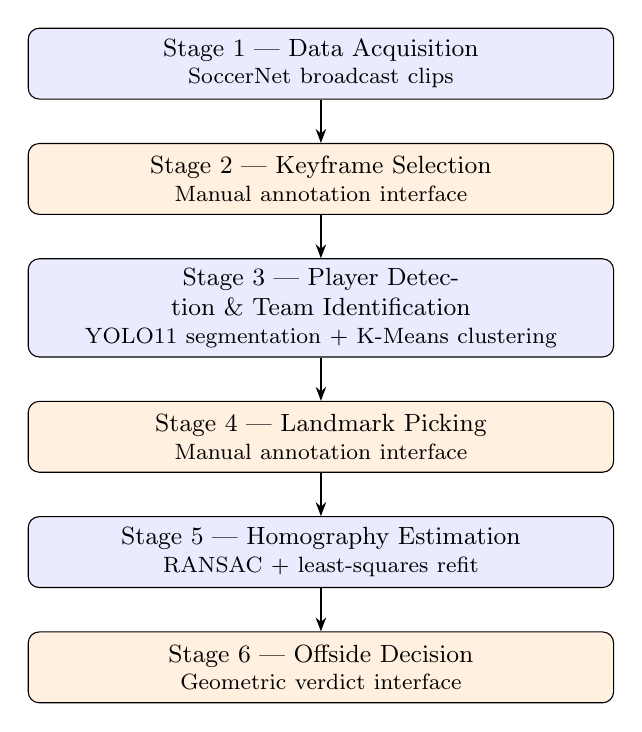
\begin{tikzpicture}[
  node distance = 0.55cm,
  auto/.style  = {rectangle, draw, rounded corners=4pt,
                  fill=blue!8, text width=7.2cm,
                  align=center, minimum height=0.9cm, font=\small},
  man/.style   = {rectangle, draw, rounded corners=4pt,
                  fill=orange!12, text width=7.2cm,
                  align=center, minimum height=0.9cm, font=\small},
  arr/.style   = {-{Stealth[length=5pt]}, thick}
]
\node[auto] (acq)  {Stage 1 — Data Acquisition\\[-1pt]
                    {\footnotesize SoccerNet broadcast clips}};
\node[man,  below=of acq]  (kf)   {Stage 2 — Keyframe Selection\\[-1pt]
                    {\footnotesize Manual annotation interface}};
\node[auto, below=of kf]   (det)  {Stage 3 — Player Detection \& Team Identification\\[-1pt]
                    {\footnotesize YOLO11 segmentation + K-Means clustering}};
\node[man,  below=of det]  (lm)   {Stage 4 — Landmark Picking\\[-1pt]
                    {\footnotesize Manual annotation interface}};
\node[auto, below=of lm]   (hom)  {Stage 5 — Homography Estimation\\[-1pt]
                    {\footnotesize RANSAC + least-squares refit}};
\node[man,  below=of hom]  (off)  {Stage 6 — Offside Decision\\[-1pt]
                    {\footnotesize Geometric verdict interface}};
\draw[arr] (acq) -- (kf);
\draw[arr] (kf)  -- (det);
\draw[arr] (det) -- (lm);
\draw[arr] (lm)  -- (hom);
\draw[arr] (hom) -- (off);
\end{tikzpicture}
\caption{Pipeline overview. Blue stages are fully automated; orange stages require operator input.}
\label{fig:pipeline_overview}
\end{figure}

The three automated stages (1, 3, and 5) run without human interaction and produce deterministic output given fixed inputs. The three manual stages (2, 4, and 6) are implemented as lightweight browser-based interfaces served by Python's built-in HTTP server, allowing the operator to interact with the pipeline from any browser without installing additional software. The deliberate inclusion of manual stages reflects the scope constraints stated in Section~\ref{sec:intro_scope}: automating keyframe selection and landmark detection are non-trivial problems in their own right, and removing them from scope allows the evaluation to focus on the accuracy of the geometric and classification components.

\section{Pipeline Stages}%
\label{sec:design_stages}

\subsection{Stage 1 — Data Acquisition}%
\label{sec:design_acq}

The input data is drawn from the SoccerNet dataset~\cite{giancola2018soccernet,deliegev2soccernet}, which provides broadcast video of professional football matches together with temporal annotations for notable events including offside decisions. Match videos are downloaded using the SoccerNet Python package, and a clip-extraction script trims each annotated offside event to a short window centred on the event timestamp. Each clip is stored as an MP4 file named with the match identifier, half, and event index, producing a collection of short broadcast clips ready for annotation.

\subsection{Stage 2 — Keyframe Selection}%
\label{sec:design_keyframe}

For each clip, the user must identify the exact frame at which the ball leaves the passer's foot, since this is the instant at which the offside condition is evaluated according to Law~11. A browser-based interface displays each extracted clip frame by frame, providing the user with buttons for single-frame stepping, ten-frame and twenty-five-frame jumps, along with a slider at the top for easier browsing. Pressing the mark button appends the current frame index to a JSON annotation file. The interface also supports skipping clips that are unsuitable, this was done because there was a number of clips in which the player who ends up receiving the ball would not be visible at the same time that the ball was played and therefore these inappropriate clips could not be evaulated under my system. The output of this stage is a mapping from each clip filename to the annotated frame index.

\subsection{Stage 3 — Player Detection and Team Identification}%
\label{sec:design_detection}

The annotated frame index obtained from the previous step is now used to export each keyframe as a JPEG image. These images are then passed to the YOLO11 object detector to detect all visible players. The segmentation variant of YOLO11 is used in preference to the plain detection variant, because it produces per-pixel masks for each detected player, which allows kit colour sampling to be restricted to body pixels rather than the rectangular bounding box region. Detection is performed in two passes to maximise recall across the full depth of the pitch. A primary pass at a confidence threshold of 0.3 collects all persons above an adaptive minimum height. A secondary pass at confidence 0.05 is then run; only detections whose bounding box centre falls in the upper portion of the frame --- the far end of the pitch, where perspective compression makes distant players appear small --- are accepted from this pass. Duplicate detections between passes are suppressed by an intersection-over-union overlap check.

For each detection, a torso crop is extracted by restricting the bounding box to the top two thirds of the player's height, done intentionally to reduce contribution of players shoes and socks which often vary in colour and could significantly effect the calculation of the clustering algorithm. Apart from that, the bounding box was also trimmed horizontally to possibly eliminate the arms and sleeves. Grass-coloured pixels are identified by computing the mean grass colour from the image in HSV colour space and excluded before colour analysis. The remaining pixels are converted to CIE Lab colour space and summarised by a six-dimensional feature vector comprising the median L*, a*, and b* values, together with three additional statistics capturing the proportion of dark pixels, the proportion of bright pixels, and a saturation proxy. This richer representation improves separation between dark and light kits that are close in hue.

K-Means clustering with $k = 2$ is then applied to the set of player feature vectors to partition players into two teams. Detections belonging to neither team (referees, partially visible players) may be reassigned or excluded at this stage. The output is a JSON file recording, for each keyframe, the set of player bounding boxes and their assigned team labels.

\subsection{Stage 4 — Landmark Picking}%
\label{sec:design_landmarks}

To estimate the homography between the image plane and the real-world pitch, a set of point correspondences must be established. A second browser-based interface displays each keyframe and allows the operator to click on visible pitch landmarks such as line intersections, corner flags, and penalty-spot markings. For each click, the operator also enters the known real-world coordinates of that landmark in the FIFA standard pitch coordinate system, in which the origin is at the pitch centre and coordinates are expressed in metres. Each click is refined to subpixel accuracy before being stored. A minimum of four correspondences are required per keyframe, since each correspondence contributes two linear constraints on $\mathbf{H}$ and the homography has eight degrees of freedom, making four the mathematical minimum for a unique solution (as derived in Section~\ref{sec:bg_geometry}); in practice, between five and ten are typically identified to over-constrain the system and improve robustness.

\subsection{Stage 5 — Homography Estimation}%
\label{sec:design_homography}

The landmark correspondences are passed as input to a homography estimation script, which uses RANSAC to establish a reliable $3 \times 3$ homography matrix $\mathbf{H}$ mapping image coordinates to real-world pitch coordinates. A reprojection threshold of 2.0\,m is used. The threshold must be calibrated to the precision achievable with manual landmark clicks at broadcast-camera scale: one pixel near the far touchline corresponds to approximately 0.06\,m in world space, so a threshold of 0.5\,m would permit only $\pm$8\,pixels of click error, which is stricter than the $\pm$10--15\,pixel localisation precision of a human operator. A threshold of 2.0\,m correctly accepts well-placed clicks at all depths of the visible pitch while still rejecting gross errors --- a misidentified landmark is typically displaced by tens of pixels, corresponding to several metres of world-space error. The final homography is then established using an ordinary least-squares refit on the RANSAC inlier set, which yields a tighter solution than the RANSAC homography alone. The quality of each estimated homography is then reported as the symmetric pixel reprojection error, calculated by mapping the original world coordinates back through $\mathbf{H}^{-1}$ and measuring the Euclidean distance to the clicked point. A validation overlay image is also produced, projecting the FIFA pitch line model into the keyframe so that alignment errors are immediately visible.

\subsection{Stage 6 — Offside Decision}%
\label{sec:design_offside}

The final stage applies the offside rule geometrically. A browser extension provides a user interface which displays each keyframe along with the player detections and their team identifications. It asks the user to choose the attacking team, the direction of attack and the attacker who ends up receiving the ball. The system then automatically identifies the second-to-last defender by projecting the leading edge of each defending player's bounding box through $\mathbf{H}$ into world coordinates and ranks the defenders by their world-space position relative to the direction of attack, the most advanced outfield defender is then selected.

With both offensive and defensive players identified, the system projects their foot positions (the lower midpoint of each bounding box) into world coordinates via $\mathbf{H}$, extracts the component along the direction of attack, and compares the two values. If the attacker's world position is further forward than the defender's, the verdict is offside; otherwise it is onside. The interface also provides the user with the margin between the two players in metres and is reported together with the verdict. An offside line is also back-projected into the image for visual verification. The verdict and all associated data are written to a JSON output file for subsequent evaluation and analysis.

\section{Design Decisions and Alternatives Considered}%
\label{sec:design_decisions}

\subsection{Choice of Object Detector}%
\label{sec:design_det_choice}

YOLO11 was selected as the player detection model because it offers a balance between being accurate and being fast, along with the availability of pretrained weights that cover the \texttt{person} class. Two-stage detectors such as Faster R-CNN~\cite{ren2015faster} were considered but rejected on both speed and accuracy grounds. Benchmarked on the same hardware used in this project (NVIDIA RTX~3060), Faster R-CNN with a ResNet-50-FPN backbone requires approximately 487\,ms per image, compared with 45\,ms for a single YOLO11x-seg pass — roughly a 10$\times$ slowdown. Critically, this speed penalty does not come with an accuracy advantage: Faster R-CNN R-50-FPN achieves approximately 37.4\% box AP on COCO~\cite{ren2015faster}, while YOLO11x-seg achieves 54.7\%~\cite{ultralytics2024yolo11}, making YOLO11x-seg both faster and more accurate on this benchmark. Although inference time is not a hard constraint for a static single-keyframe pipeline, the combination of lower accuracy and 10$\times$ higher latency gives no justification for choosing Faster R-CNN. Of the  one-stage detectors, YOLO11 is a state of the art for the YOLO family~\cite{ultralytics2024yolo11} and is more accurate than its predecessors on the COCO benchmark. The largest segmentation variant, YOLO11x-seg, was selected over smaller variants. YOLO11x achieves the highest reported box mAP of 54.7\% on the COCO benchmark among all YOLO11 variants~\cite{ultralytics2024yolo11}. To confirm this advantage on the actual dataset, YOLO11n-seg, YOLO11m-seg, and YOLO11x-seg were each run at a confidence threshold of 0.3 across all 164 annotated keyframes. YOLO11x-seg produced a mean of 15.3 detections per frame compared with 14.5 for both YOLO11m-seg and YOLO11n-seg, yielding on average 0.8 additional detections per frame and outperforming YOLO11m-seg in the majority of frames. The additional detections are concentrated in distant or partially occluded players at the far end of the pitch, precisely the cases where a smaller model loses recall. This empirical advantage was also observed qualitatively during development, where YOLO11m-seg frequently missed players in the far half of the pitch (see Section~\ref{sec:impl_challenges}). The per-pixel segmentation masks produced by the segmentation variant additionally allow kit colour sampling to be restricted to pixels belonging to the player's body, reducing contamination from background grass and improving team identification accuracy.

\subsection{Team Identification Method}%
\label{sec:design_teamid_choice}

Kit colour clustering in CIE Lab colour space was chosen as the team identification method in preference to several alternatives. A deep feature-based approach, in which a pretrained \gls{cnn} is used to extract appearance embeddings for each player, would require either fine-tuning on labelled football data or a zero-shot embedding model, both of which add considerable complexity and computational cost. Benchmarked on the project hardware, passing a batch of 19 player crops through a ResNet-50 feature extractor requires approximately 37\,ms, compared with 1.6\,ms for K-Means clustering on the same 19 players — a 23$\times$ overhead with no labelled football data to demonstrate a compensating accuracy gain. Colour-based clustering is sufficient because the Laws of the Game require teams to wear distinct kits. CIE Lab was chosen over RGB or HSV because its Euclidean distance is perceptually uniform, producing more stable K-Means boundaries across varying lighting conditions. The six-dimensional feature vector, which adds brightness and saturation statistics to the three Lab channel medians, was found to improve discrimination between kits that are spectrally similar but differ in lightness.

\subsection{Manual Keyframe Selection}%
\label{sec:design_kf_choice}

Keyframe selection is performed manually. Automated ball detection is unreliable in broadcast footage where the ball is frequently occluded or blurred, and an incorrect keyframe directly corrupts the verdict. The operator time cost of 10--30 seconds per event is a justified trade-off for guaranteed correctness.

\subsection{Manual Landmark Picking}%
\label{sec:design_landmark_choice}

Pitch landmark identification is similarly performed manually. Automated approaches such as Hough-based line detection or semantic segmentation are sensitive to player occlusion and variable broadcast angles. Manual picking allows the operator to select the most reliable landmarks per frame, producing higher-quality correspondences than a fixed automated method.

\subsection{Foot-Level Projection and World-Space Defender Ranking}%
\label{sec:design_projection_choice}

The pitch position for each player is the projection of the leading-edge foot point of their bounding box: the bottom corner on the side facing the direction of attack. This follows the geometric interpretation of Law~11, which checks the body part closest to the goal line, and avoids the overestimation that would result from using the centroid.

The most advanced defender is identified by ranking players in world space after projecting through $\mathbf{H}$, avoiding the perspective distortion that makes image-space ranking unreliable on oblique cameras. This adds no computational cost since the homography has already been computed.

\chapter{Implementation}%
\label{chp:implementation}

\section{Tooling, Environment, and Data Acquisition}%
\label{sec:impl_tooling}

All stages within the pipeline are developed entirely in Python~3. OpenCV is used throughout for image processing including reading images, colour space conversion, and homography computation. Player detection and segmentation are performed using the Ultralytics library with the YOLO11x-seg pretrained weights. Player kit colour is identified by running K-Means clustering using scikit-learn. Clip extraction relies on FFmpeg invoked as a subprocess, and the SoccerNet Python package is used to download match video files and to parse event annotations. The three annotation interfaces are served by Python's built-in \texttt{http.server} module and share a common architecture: a single-page HTML application is served locally, the browser communicates with the Python backend via fetch requests to JSON endpoints, and state is written to disk only on operator confirmation. Completed frames are loaded on startup and skipped, so any session can be interrupted and resumed without loss of work. All intermediate outputs --- keyframe indices, player detections, landmark correspondences, homography matrices, and offside verdicts --- are stored to disk as JSON files, so that every stage can be rerun independently.

Match footage is obtained through the SoccerNet API. For each downloaded match, the event annotation file is parsed to identify all offside events, each carrying a timestamp in milliseconds. For each offside event a short clip is then extracted using FFmpeg: 10 seconds before the timestamp and 25 seconds after, summing up to a 35-second window which would possibly contain both the live moment and any broadcast replay of the offside event. For any already extracted clip, it is skipped and not extracted again to avoid any redundancy.

\section{Keyframe Annotation Interface}%
\label{sec:impl_keyframe}

From each extracted clip the operator must identify the single frame at which the ball leaves the passer's foot. A browser-based annotation interface (\texttt{annotate\_keyframes.py}, port~5000) was developed for this purpose. It loads all frames from a clip into memory using OpenCV, serves individual frames as base64-encoded JPEGs, and provides single-frame, ten-frame, and twenty-five-frame navigation together with a timeline scrubber. The operator marks the chosen frame with a button press or keyboard shortcut, or skips the clip entirely if the relevant players are not visible. The annotation state is persisted after every user interaction, allowing the operator to resume an interrupted session at any point. A separate script then exports the marked JPEG keyframe from each clip.

\section{Player Detection and Team Identification}%
\label{sec:impl_team_id}

YOLO11x-seg is run on each keyframe to produce bounding boxes and per-pixel segmentation masks for all detected persons. The segmentation variant is used because the mask allows kit colour extraction to sample only pixels belonging to the player's body, rather than the background included in a plain bounding box crop.

Detection is performed in two passes to balance precision and recall across the depth of the pitch. A primary pass at confidence 0.3 with an NMS IoU threshold of 0.7 collects all person detections above an adaptive minimum height. The 0.3 confidence floor removes low-quality detections while retaining players at medium distances; the 0.7 NMS IoU threshold (the Ultralytics default) suppresses duplicate boxes of the same player without merging adjacent players standing close together. The minimum height threshold is set adaptively based on the median detected player height in the primary pass: if the median is below 45 pixels (indicating a wide-angle view with many distant players), the minimum is set to 20 pixels to retain small far-end detections; otherwise it is set to 40 pixels to filter non-player noise. These height values were calibrated empirically against the annotated keyframe set to balance retention of legitimate far-end players against rejection of noise detections. A secondary pass at confidence 0.05 is then run; only detections whose bounding box centre falls in the upper \texttt{top\_zone} fraction of the frame are accepted, targeting the far end of the pitch where perspective compression makes distant players appear smaller than the primary pass minimum height. Duplicate detections between passes are suppressed by an IoU overlap check with a threshold of 0.4 --- looser than the NMS threshold to account for the fact that far-end boxes are small and overlap estimates are noisier. Detections near the touchline, in image corners, or at the very bottom of the frame are subsequently classified as non-pitch personnel and excluded from the team identification step. Evaluated across the full 164 annotated keyframes in the dataset, the secondary pass contributed 499 additional detections that the primary pass missed, affecting 139 of 164 frames (84.8\%). On affected frames the secondary pass recovered an average of 3.6 additional players per frame, with a maximum of 15 in a single frame. These recovered players are disproportionately defenders near the far end of the pitch, whose position along the offside line makes their inclusion critical to a correct verdict.

For each remaining detection, a torso region of interest is defined by restricting the crop vertically to between 20\% and 60\% of the bounding box height, skipping the head and legs. A horizontal trim of 18\% is applied to each side of the crop to reduce contamination from arm skin and sleeve edges. Pixels in this region whose colour in \gls{hsv} space falls within the grass green range are excluded; the grass colour is estimated from the image by masking the field and computing the mean BGR value. \gls{hsv} is used at this stage because grass occupies a compact, well-defined hue band that can be isolated with a simple range check, and the binary grass/not-grass decision does not require perceptually uniform distances. The remaining pixels are converted to CIE Lab for feature extraction: unlike \gls{hsv}, CIE Lab is perceptually uniform, meaning Euclidean distances correspond to perceived colour differences, which is a necessary property for K-Means clustering to group players by visually similar kit colours rather than by arbitrary numerical proximity. The pixels are summarised by the six-dimensional feature vector shown in Listing~\ref{lst:feature}.

\begin{lstlisting}[language=Python, caption={Construction of the six-dimensional kit colour feature vector.}, label={lst:feature}]
median_L = np.median(L)
median_a = np.median(a)
median_b = np.median(b)
dark_ratio  = np.mean(L < 80)
bright_ratio = np.mean(L > 150)
sat_proxy = np.median(np.sqrt((a - 128)**2 + (b - 128)**2))
size_factor = min(1.0, (height * width) / 8000)
return np.array([median_L, median_a, median_b,
                 dark_ratio * 100 * size_factor,
                 bright_ratio * 100, sat_proxy])
\end{lstlisting}

Three aspects of the feature vector construction require explanation. First, the saturation proxy is computed as $\text{median}\!\left(\sqrt{(a^* - 128)^2 + (b^* - 128)^2}\right)$ rather than simply $\sqrt{(a^*)^2 + (b^*)^2}$: OpenCV encodes CIE Lab so that the achromatic (neutral grey) point lies at $(a^*, b^*) = (128, 128)$, not at the origin, so the subtraction re-centres the distance measurement at the true neutral point. Without this correction the saturation proxy would measure distance from a corner of the colour space rather than from achromatic, producing incorrect saturation estimates for dark kits. Second, the \texttt{size\_factor} scales the dark-ratio dimension by $\min(1,\, h \times w\, /\, 8000)$, where $8000\,\text{px}^2$ corresponds approximately to the bounding box area of a player at mid-distance in a broadcast frame ($\approx 90 \times 90$\,px). Small distant players have a proportionally larger fraction of background pixels in their crop, producing noisier colour estimates; down-weighting the dark-ratio dimension for small boxes reduces their influence on the cluster centroids. Third, grass pixels are excluded using an HSV mask with hue range $[35^\circ, 85^\circ]$, saturation above 40 and value above 40 (both on OpenCV's 0--255 scale, where saturation measures colour intensity and value measures brightness, so these thresholds exclude near-grey and near-black pixels respectively), which covers the full range of natural and broadcast-lit grass colours while avoiding false positives on yellow or white kit elements.

Prior to clustering with K-Means, players likely to belong to referees, goalkeepers, or other non-outfield categories are pre-flagged and excluded from clustering. A player is pre-flagged under two conditions: (i)~their L* is below 50 (nearly black), indicating a referee kit, provided they are not chromatically consistent with at least two other players (which would suggest a dark team kit rather than an official); or (ii)~their L* is below 100 and their chromaticity is below a saturation of 13, capturing the low-saturation dark grey typical of referees. A separate check flags any player whose $(a^*, b^*)$ chromaticity has fewer than two similar neighbours within a radius of 15 units in $a^*b^*$ space as colour-isolated, removing outlier kits not shared by at least two others. A mini-team rescue pass prevents a small team visible in only three players from being entirely flagged: if three or more isolated players are mutually within a chroma radius of 22 they are restored to the clustering pool, as they form a coherent group rather than scattered officials.

All numeric thresholds (torso crop boundaries, HSV grass mask, OTH pre-flag bounds, neighbourhood radii) were determined empirically via iterative visual inspection. Per-parameter ablation is infeasible without per-player ground-truth labels, which SoccerNet does not provide; instead the thresholds were tuned during initial development on a small subset of frames and then held fixed for the full 164-frame evaluation. The 2.0\% end-to-end team misidentification rate measured across that broader, untouched set indicates that the chosen values generalise rather than overfit to the development subset.

With the remaining players, K-Means with $k=2$ is applied to the standardised feature vectors. The choice of $k=2$ reflects the domain constraint that exactly two outfield teams are present in any match. Setting $k=3$ to absorb referees and goalkeepers directly was considered but rejected: because kit colour variation within a team (due to lighting, shadow, and distance) can exceed the colour difference between a referee's kit and one of the teams, a third cluster frequently captures within-team variation rather than officials, producing a degenerate split. Pre-flagging non-outfield personnel before clustering and enforcing $k=2$ on the remainder is more robust. Before clustering, features are normalised with \texttt{StandardScaler} and the $a^*$ and $b^*$ chroma channels are then multiplied by 1.8 to re-emphasise hue over brightness. This is necessary because K-Means implicitly assumes clusters of equal isotropic variance in feature space, so any dimension with greater raw spread tends to dominate the cluster boundary regardless of how discriminative it is; in football broadcasts the L* (brightness) channel varies strongly with shadow and camera angle while shirt hue is consistent, so unweighted clustering reliably splits on brightness rather than team colour. The 1.8 weight was selected empirically and balances chroma dominance without overwhelming the remaining dimensions. K-Means is run five times with different random seeds and the result with the most balanced cluster sizes is retained; the balance score is $\min(c_0, c_1)\,/\,\max(c_0, c_1)$, where $c_0$ and $c_1$ are the cluster sizes, giving 1.0 for a perfect 50/50 split. This multi-start strategy guards against the known sensitivity of K-Means to initialisation, particularly when the two team colours are close together in Lab space. The resulting team assignments for a representative keyframe are shown in Figure~\ref{fig:team_id}.

\begin{figure}[h]
  \centering
  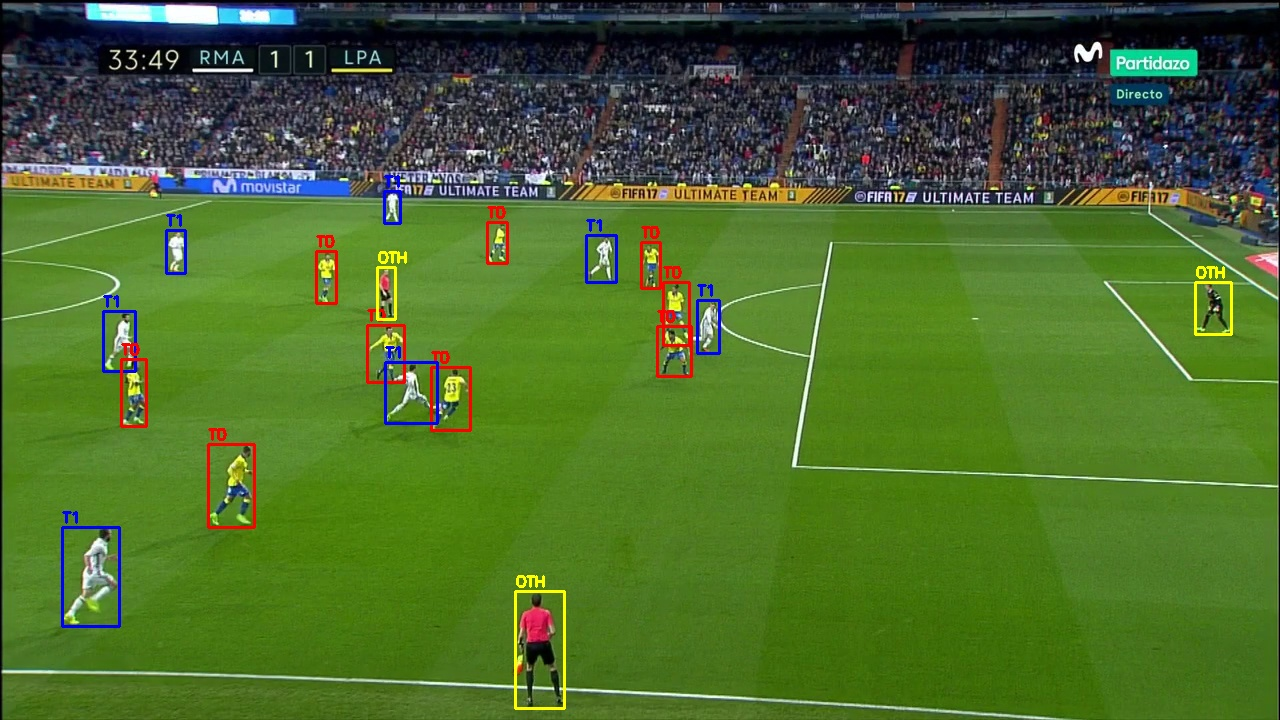
\includegraphics[width=0.9\linewidth]{content/chapters/4_implementation/figures/team_identification_figure.jpg}
  \caption{YOLO11x-seg detections with K-Means clustering team assignment. Blue boxes indicate Team~1, red boxes Team~0, and yellow indicates an OTH (referee/goalkeeper/non-outfield detection). Labels show the detection index and cluster assignment.}
  \label{fig:team_id}
\end{figure}

\section{Homography Estimation}%
\label{sec:impl_homography}

Pitch landmark correspondences are collected through a browser-based interface (\texttt{pick\_points.py}, port~5001). The interface serves each keyframe image and captures click coordinates from the browser, displaying a live table of entered correspondences. Each recorded point is further refined to subpixel precision using OpenCV's \texttt{cornerSubPix} function, which iteratively repositions the click to the nearest intensity-gradient corner within a $7\times7$ pixel search window. The iterative refinement runs for at most 30 iterations and terminates early if the point moves less than 0.01 pixels between steps, balancing precision against computational cost. Refinement is skipped if the click falls within 2 pixels of the image edge, where the search window would extend outside the image boundary. The operator then selects the corresponding landmark on an interactive pitch diagram to provide the real-world coordinate, and must submit at least four correspondences before the frame is accepted --- four being the theoretical minimum: $\mathbf{H}$ has eight degrees of freedom (nine matrix entries, minus one for the scale ambiguity), and each point correspondence contributes exactly two independent linear constraints, so four correspondences are needed to make the system fully determined.

The homography is estimated using a two-stage process, illustrated in Listing~\ref{lst:homography}. The first pass applies RANSAC with a reprojection threshold of 2.0\,m to identify a consistent inlier set. RANSAC was preferred over the alternative robust estimator LMedS (\texttt{cv2.LMEDS}), which minimises the median squared residual and requires no threshold, because the explicit threshold of RANSAC can be reasoned about directly in terms of expected click precision, making the choice transparent and adjustable; LMedS offers no equivalent handle. This threshold was chosen to match the precision achievable with manual landmark clicks: at the far touchline, where perspective compression is greatest, one pixel corresponds to approximately 0.06\,m, making the practical click precision of $\pm$10--15\,pixels equivalent to $\pm$0.6--0.9\,m of world-space error. A threshold of 2.0\,m therefore accepts all reasonably-placed clicks while still rejecting gross outliers such as misidentified landmarks. The second pass refits $\mathbf{H}$ from only the RANSAC inlier set via ordinary least squares (\texttt{method=0}), which is the maximum-likelihood estimate under Gaussian noise and produces a tighter solution than the RANSAC homography alone.

\begin{lstlisting}[language=Python, caption={Two-pass homography estimation: RANSAC followed by least-squares refit on inliers.}, label={lst:homography}]
H_ransac, mask = cv2.findHomography(
    image_pts, real_pts, cv2.RANSAC,
    ransacReprojThreshold=2.0)

inliers_mask = mask.ravel().astype(bool)
if inliers_mask.sum() >= 4:
    H, _ = cv2.findHomography(
        image_pts[inliers_mask],
        real_pts[inliers_mask],
        method=0)   # ordinary least squares
\end{lstlisting}

A homography is defined only up to scale, meaning $\mathbf{H}$ and $-\mathbf{H}$ represent the same projective transformation. However, only one sign produces valid (positive projective denominator) projections for points on the physical pitch plane; the opposite sign maps those points to the geometrically mirrored half-space, producing sign-flipped world coordinates. After estimation, the sign of $\mathbf{H}$ is normalised by checking the projective denominator at the centroid of the picked image points: if the denominator is negative, $\mathbf{H}$ is negated. This step is necessary to guarantee that world-space $x$-coordinates produced by the system carry the correct sign for the offside comparison.

A final quality gate is applied before a frame is passed to the offside checker: a $12 \times 8$ grid of sample points is projected through $\mathbf{H}$ across the player zone of the image, and the fraction with a non-positive projective denominator is recorded. Frames where more than 15\% of the player zone produces invalid projections are automatically excluded, as the homography is not well-conditioned enough to support reliable player position estimates across the full pitch. The 15\% threshold was determined empirically as the value that correctly excluded near-singular homographies while retaining all frames with geometrically valid calibrations.

The quality of each estimated homography is reported as the symmetric pixel reprojection error: the known world coordinates of each correspondence are transformed back into the image via $\mathbf{H}^{-1}$ and the Euclidean distance to the original click position is measured. A validation overlay is also rendered for each keyframe by projecting the full FIFA pitch line model through $\mathbf{H}^{-1}$; the resulting lines should align with the visible pitch markings, making any gross calibration error immediately apparent, as illustrated in Figure~\ref{fig:homography_validation}.

\begin{figure}[h]
  \centering
  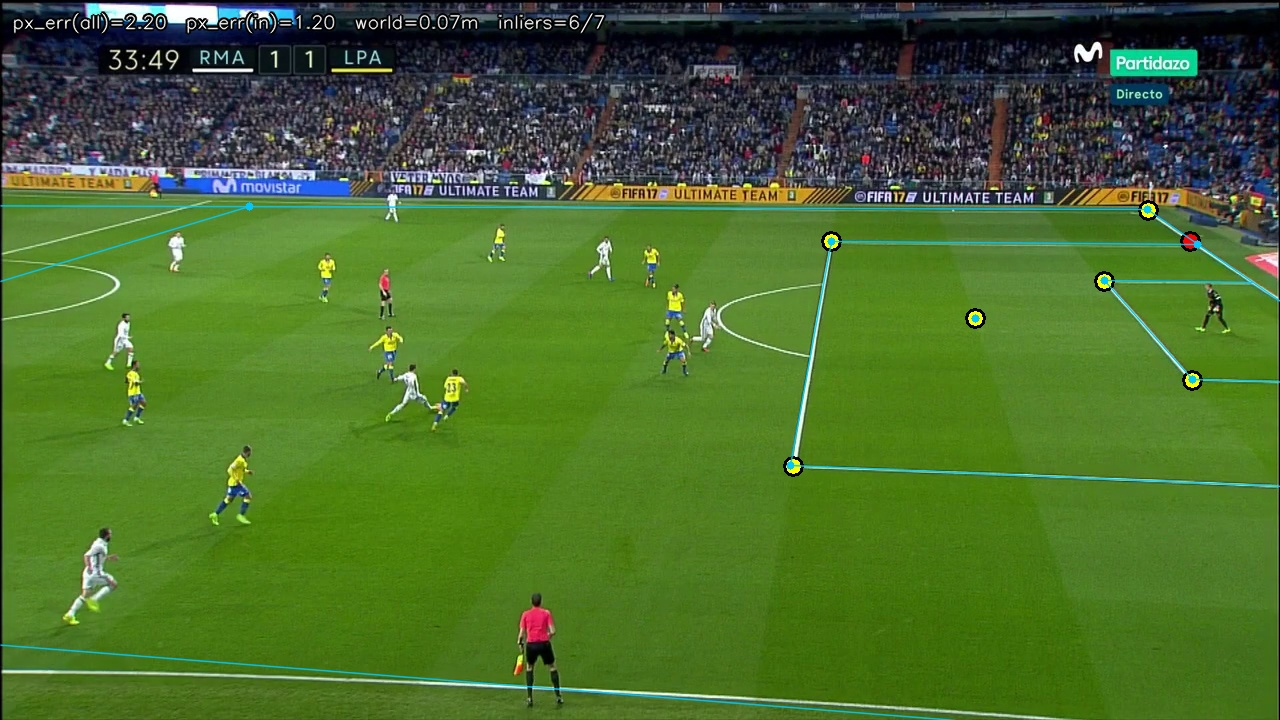
\includegraphics[width=0.9\linewidth]{content/chapters/4_implementation/figures/homography_validation_figure.jpg}
  \caption{Homography validation overlay: the FIFA pitch line model is projected back into the image via $\mathbf{H}^{-1}$ and rendered in cyan. Close alignment with the visible pitch markings confirms a consistent calibration.}
  \label{fig:homography_validation}
\end{figure}

\section{Offside Decision}%
\label{sec:impl_offside}

The offside checker interface (port~5002) accepts the operator-specified attacking team, direction of attack, and attacker index. All defending players' foot positions are projected through $\mathbf{H}$ into world coordinates; before ranking, any defender whose projected position falls outside the FIFA pitch boundary ($|X| \leq 52.5$\,m, $|Y| \leq 34$\,m with a small margin) is excluded, as this indicates a touchline steward or pitch-side official that YOLO has detected as a person rather than an outfield player. The most advanced remaining defender along the direction of attack is taken as the second-to-last defender.

The foot position used for both attacker and defender is the bottom corner of the bounding box on the side facing the direction of attack: the right-edge foot $(x_2, y_2)$ when attacking right, and the left-edge foot $(x_1, y_2)$ when attacking left. This measures the leading edge of each player's ground contact region, consistent with the body-part interpretation of Law~11. Both points are projected through $\mathbf{H}$ to give world coordinates $(X_{\text{att}},\, Y_{\text{att}})$ and $(X_{\text{def}},\, Y_{\text{def}})$. The signed margin $m = d\cdot(X_{\text{att}} - X_{\text{def}})$ is then computed, where $d \in \{+1, -1\}$ encodes the direction of attack as detected from the homography axis orientation. A positive $m$ indicates the attacker is ahead of the defender (offside); a negative $m$ gives onside. The magnitude $|m|$ is reported in metres. The offside line is rendered by inverting $\mathbf{H}$ at the defender's world $x$-coordinate to obtain two image-space points, which are connected with a line overlay across the full height of the frame.

\section{Challenges Encountered}%
\label{sec:impl_challenges}

Several implementation problems arose that required significant revision of the initial design.

\textbf{Insufficient player detection.} The initial implementation used YOLO11m, which frequently missed detections in the far half of the pitch where distant players appear small. Replacing it with YOLO11x-seg improved recall for small and partially occluded players: across all evaluation keyframes, YOLO11x-seg produced on average 0.8 additional detections per frame. The segmentation masks further allowed colour extraction to sample only pixels inside the player's outline rather than the rectangular bounding box crop.

\textbf{Kit colour contamination.} Early team identification used the median Lab colour of a simple bounding box crop, which included arm skin and shorts contamination. Three refinements addressed this: a vertical restriction to the upper-middle torso region, an 18\% horizontal trim, and grass-colour exclusion via HSV masking. The combined effect is reflected in the evaluation: team misidentification accounted for only 3 of the 150 clean events (2.0\%), attributable to spectrally similar kits rather than contamination.

\textbf{OTH classifier over-flagging outfield players.} The initial approach used simple luminance thresholds to identify referees and goalkeepers, which frequently misclassified outfield players in dark or unusual kits as officials. Outlier detection was rebuilt around the modified Z-score $\tau = \tilde{d} + 3.5 \cdot 1.4826 \cdot \mathrm{MAD}$~\cite{iglewicz1993outliers}, where $\tilde{d}$ is the median centroid distance and $1.4826$ is the standard consistency factor relating the \gls{mad} (a robust, outlier-resistant measure of spread) to the standard deviation of a Gaussian. A player is flagged OTH only when their distance exceeds $\tau$ \emph{and} they are not clearly assigned to one team. A bimodal chroma refit handles frames where K-Means splits on brightness rather than hue.

\textbf{Insufficient landmark coverage.} The initial landmark set (halfway line, penalty box corners, centre circle) proved insufficient for frames where the camera is near one end of the pitch. The set was extended to include 6-yard box corners, goalpost bases, and corner flags, which are visible in nearly all valid broadcast frames and improved both inlier count and reprojection error.

\textbf{RANSAC threshold calibration.} The initial threshold of 0.5\,m proved too strict: at the far touchline, one pixel corresponds to approximately 0.06\,m, making 0.5\,m equivalent to only $\pm$8 pixels of tolerated click error. Since manual clicks achieve $\pm$10--15 pixels, the threshold routinely rejected correctly-placed correspondences, leaving the homography under-constrained where the offside line typically lies. Relaxing to 2.0\,m accommodates realistic click imprecision while still rejecting gross misidentifications --- a wrongly-clicked landmark is typically displaced by 50--100 pixels or more. Across 162 calibrated frames this produced a mean inlier ratio of 94.5\%, confirming that most correspondences are accepted.

\textbf{Image-space defender ranking and reprojection error metric.} Ranking by image-space x-coordinate fails on oblique cameras; projecting foot positions through $\mathbf{H}$ resolves this. World-space residuals in metres were replaced by the symmetric pixel reprojection error of Section~\ref{sec:impl_homography}, which is consistent at all depths.

\chapter{Evaluation}%
\label{chp:evaluation}

% Per FYP guidelines, this chapter is critical. Required content:
%   - Justify why each test is relevant (cite literature on similar systems).
%   - Demonstrate whether the system works as intended (be honest if it does not).
%   - Comprehensible summaries of all critical test results.
%   - Critical evaluation of strengths AND weaknesses.
%   - Comparison with published work where available.

\section{Evaluation Methodology}%
\label{sec:eval_methodology}

% TODO: dataset, ground truth, metrics. Justify choices using literature.

\section{Player Detection Accuracy}%
\label{sec:eval_detection}

% TODO: e.g.\ mAP, precision, recall on annotated SoccerNet samples.

\section{Team Identification Accuracy}%
\label{sec:eval_team_id}

% TODO: confusion matrix / accuracy on annotated keyframes.

\section{Homography Reprojection Error}%
\label{sec:eval_homography}

% TODO: distribution of reprojection error in metres across keyframes.

\section{End-to-End Offside Verdicts}%
\label{sec:eval_offside}

% TODO: agreement with \gls{var} / human judgement on annotated events.

\section{Comparison with Existing Work}%
\label{sec:eval_comparison}

% TODO: published systems and where this work sits relative to them.

\chapter{Future Work}%
\label{chp:future_work}

% Per FYP guidelines: ideas that evolved beyond the original scope, and
% partial work that could be extended. Examples relevant to this project:
% automatic ball-played detection (removing manual keyframe step),
% multi-camera setups, real-time inference, broader event detection
% (corners, fouls, goals).

\textit{To be written.}

\chapter{Conclusions}%
\label{chp:conclusions}

The purpose of this final year project was to design, implement, and evaluate a modular computer vision pipeline capable of producing offside verdicts from broadcast football footage, without requiring the dedicated multi-camera infrastructure used by professional \gls{var} systems. The seven objectives stated in Section~\ref{sec:intro_aims} have each been addressed and fulfilled, demonstrating that the core aim is indeed achievable.

\section{Review of Objectives}%
\label{sec:conc_objectives}

The first three objectives focused on data acquisition and preparation. Matches and associated ground-truth annotations were gathered from SoccerNet across six competitions and multiple seasons. A total of 457 offside clips were extracted and filtered, each trimmed to a 35-second window around the annotated event. A browser-based keyframe annotation interface allowed the operator to identify the exact frame at which the ball was played; out of the 457 clips, 164 yielded usable keyframes and 293 were treated as unsuitable.

The fourth objective was player detection and team assignment. The keyframes were analysed using the YOLO11x-seg algorithm. On average 18.8 players were detected per frame, with no frame producing zero detections. The team was assigned using a 6D CIE Lab feature vector which was clustered using K-Means, successfully assigning the teams in most of the 164 cases. Team misidentification, attributable to spectrally similar kits, accounted for three of the 22 disagreements on the clean evaluation set; the remaining 19 disagreements were marginal or moderate cases within the geometric uncertainty of the calibration.

The fifth objective was to estimate a homography. A two-pass RANSAC with least-squares refit achieved a mean symmetric pixel reprojection error of 1.00\,px across the 150 retained calibrated frames (85.3\% below 2\,px), corresponding to a world-space uncertainty of approximately 15--25\,cm.

The sixth objective was to evaluate the offside condition geometrically. On the 150 clean evaluation events, overall agreement with SoccerNet annotations was 85.3\%; for the 92 confident events (margin $>$0.5\,m), agreement was \textbf{91.3\%}, and for clear cases (margin $>$1.0\,m) agreement was 97.4\%.

The seventh objective was to evaluate overall accuracy and identify failure modes. The analysis classified the failures into three categories: frames excluded by the homography quality filter (5 frames with reprojection error exceeding 3.2\,px), team misidentification (three cases), and marginal or moderate measurement uncertainty (19 cases with margin $\leq$1.0\,m).

\section{Principal Conclusions}%
\label{sec:conc_principal}

In conclusion, a system that relies entirely on broadcast footage for offside detection is practical at acceptable levels of accuracy. The almost complete agreement on the clear cases demonstrates that the geometric pipeline is fundamentally correct. In cases where the margin is clearly significant enough, the system is almost guaranteed to make the right call. The drop in agreement at sub-0.5\,m cases is not necessarily a flaw of the algorithm, but rather a mix of both limitations due to a single camera broadcast, and also cases in which the player was actually just slightly onside but the referee flagged it as offside due to the tight margin between the attacker and defender, to which linesmen are prone. 

The system compares favourably with the only comparable end-to-end published result. Uchida \textit{et~al.}\ reported an F1 score of 63.1\% using two fixed calibrated cameras on 20 clips~\cite{uchida2021offside}; the present system achieves a 91.3\% agreement rate on confident cases from a single broadcast feed across a substantially larger evaluation set.

The major challenges to the application of the technique remain: keyframe selection, pitch landmark picking, and the offside checker interaction. These steps are critical to the accuracy of the verdict. An incorrect keyframe directly invalidates the result and their automation should be the main focus of future development. The geometric and detection components of the pipeline are sufficiently accurate that, were these manual steps automated, a fully deployable system would be within reach.

\section{Closing Remarks}%
\label{sec:conc_closing}

The work presented in this final year project demonstrates that the gap between the precision available to elite football through \gls{var} and the information available from a standard broadcast feed is narrower than it might appear. A system built from publicly available tools, operating on footage that already exists for the vast majority of competitive matches, can produce geometrically grounded offside verdicts with high reliability for cases where the margin is large. Closing the remaining gap, automating the manual stages, integrating body keypoint precision, and validating against geometric ground truth are all engineering problems that this work has laid the foundation for.


\printbibliography[title=References]

\appendix{}

\chapter{User Guide}%
\label{app:user_guide}

% TODO: how to run the pipeline end-to-end (download SoccerNet metadata,
% scan offsides, download videos, extract clips, annotate keyframes,
% run team identification, pick pitch points, run offside checker).

\chapter{Source Code Structure}%
\label{app:code}

The complete source code is provided on the accompanying digital media. This appendix describes the layout of the project directory and the role of each file. Full source listings are not included in this report in accordance with the FYP guidelines.

\section*{Top-Level Directory}

\begin{tabularx}{\linewidth}{lX}
\hline
File / Directory & Purpose \\
\hline
\texttt{Makefile} & Automates the non-interactive pipeline stages. \\
\texttt{scan\_offsides.py} & Ranks available SoccerNet games by offside event count to assist game selection. \\
\texttt{download\_videos.py} & Downloads 720p match video files from SoccerNet for the configured game list. \\
\texttt{extract\_clips.py} & Extracts 35-second MP4 clips around each annotated offside event. \\
\texttt{annotate\_keyframes.py} & Browser interface (port 5000) for selecting the pass frame in each clip. \\
\texttt{export\_keyframes.py} & Exports the annotated frame from each clip as a JPEG image. \\
\texttt{team\_identification.py} & YOLO11x-seg detection and K-Means team assignment on all keyframes. \\
\texttt{pick\_points.py} & Browser interface (port 5001) for entering pitch landmark correspondences. \\
\texttt{compute\_homography.py} & Estimates homography matrices from landmark correspondences. \\
\texttt{offside\_checker.py} & Browser interface (port 5002) for reviewing and recording offside verdicts. \\
\texttt{eval/} & Evaluation scripts used to justify the Chapter~5 parameter choices (two-pass detection, NMS threshold, chroma weight). \\
\texttt{static/ui.css} & Shared stylesheet served to all three browser interfaces. \\
\hline
\end{tabularx}

\section*{Data Directory}

All pipeline inputs and outputs are stored under \texttt{data/}. This directory is not included on the digital media (video files are large); it is recreated by running the pipeline.

\begin{tabularx}{\linewidth}{lX}
\hline
Path & Contents \\
\hline
\texttt{data/soccernet/} & Downloaded SoccerNet annotation files and match videos. \\
\texttt{data/clips/} & Extracted MP4 clips, one per annotated offside event. \\
\texttt{data/keyframes.json} & Maps each clip filename to its annotated frame index. \\
\texttt{data/keyframes/} & Exported JPEG keyframe images. \\
\texttt{data/player\_detections.json} & Bounding boxes, team labels, and foot positions per keyframe. \\
\texttt{data/team\_identification/} & Visualisation images with colour-coded team bounding boxes. \\
\texttt{data/homography\_points.json} & Image--world landmark correspondences per keyframe. \\
\texttt{data/homography\_matrices.json} & Estimated $3\times3$ homography matrices and reprojection errors. \\
\texttt{data/homography\_validation/} & Validation overlay images with projected pitch line model. \\
\texttt{data/offside\_verdicts.json} & Recorded verdicts, margins, and metadata per event. \\
\texttt{data/offside\_results/} & Annotated keyframe images with offside line and verdict overlay. \\
\texttt{data/detection\_comparison/} & Side-by-side visualisations from the two-pass detection evaluation script. \\
\texttt{data/team\_identification\_debug.json} & Per-player Lab feature dump written by \texttt{team\_identification.py} in debug mode; read by \texttt{eval/test\_chroma\_weight.py}. \\
\hline
\end{tabularx}

\section*{Report Directory}

\begin{tabularx}{\linewidth}{lX}
\hline
Path & Contents \\
\hline
\texttt{report/dissertation/} & LaTeX source for this final year project. \\
\texttt{report/dissertation/main.tex} & Root document; includes all chapters and configuration. \\
\texttt{report/dissertation/content/chapters/} & One subdirectory per chapter containing the \texttt{.tex} source. \\
\texttt{report/dissertation/content/appendices/} & Appendix source files. \\
\texttt{report/dissertation/references.bib} & BibTeX reference database. \\
\hline
\end{tabularx}

\section*{Dependencies}

The pipeline was developed and tested under the following environment:

\begin{tabularx}{\linewidth}{lX}
\hline
Component & Version \\
\hline
Python & 3.11 \\
ultralytics & 8.4.19 \\
OpenCV (\texttt{opencv-python}) & 4.13.0 \\
scikit-learn & 1.8.0 \\
NumPy & 2.3.5 \\
PyTorch & 2.5.1 \\
FFmpeg & 7.x \\
Operating system & Ubuntu 22.04 (WSL2 on Windows 11) \\
\hline
\end{tabularx}


\end{document}
